%%% compile it with pdflatex
\documentclass[a4paper]{article}
\usepackage[T1]{fontenc}
\usepackage[utf8]{inputenc}
\usepackage{lmodern}
\usepackage{fancybox}
\usepackage{graphicx}

\begin{document}

\title{2APL: A Practical Programming Language and Platform for Multi-Agent Systems}
 
\author{Beltran Borja Fiz, Fabrizio De Santis, Marcos Gabarda\\
\small \texttt{\{beltran.borja.fiz, fabrizio.de.santis, marcos.gabarda\}@est.fib.upc.edu}\\
\\
Multi-Agent Systems Course\\
Master in Artificial Intelligence\\
Universitat Polit\`ecnica de Catalunya}
\date{\today}

\newenvironment{fminipage}%
  {\begin{Sbox}\begin{minipage}}%
  {\end{minipage}\end{Sbox}\fbox{\TheSbox}}


\maketitle

\tableofcontents

\section{Introduction} %%%%%%% BORJA HERE

Borja here: introduce 2apl with history

\section{2APL Language} %%%%%%% BORJA HERE

Introduce prolog + blockworld example
\\
2APL distinguishes itself from other agent-oriented programming
languages by realizing an effective integration of declarative and
imperative style programming.
The declarative style programming supports the implementation of
the mental state of agents allowing them to reason about their
mental states and update them accordingly.
The imperative style programming supports the implementation of
processes allowing programming constructs to implement both the
flow of control as well as mechanisms such as procedure call,
recursion, plan revision, and interface to existing imperative
programming languages.


\subsection{Syntax and operational semantics} %%%%%%% FABRIZIO HERE

There are two distinguished set of programming constructs for defining either a multi-agent system or individual agents.

\subsubsection{Multi-agent system specification} %%%%%%% FABRIZIO HERE

A multi-agent system is specified by a set of couples specifying each agent of the society and a set of environments they have access to. A formal specification of a multi-agent system is provided in Figure~\ref{fig:ebnf_mas}. An example for the blockworld environment described above is provided in ~\ref{ex_blockworld} where the agent \texttt{harry} and \texttt{sally} are defined both having access to the \texttt{blockworld} environment.

\begin{figure}[htbp]
\begin{verbatim}
<MAS_Prog>     := ( <agentname> ``:'' <filename> [<int>]
                   [<environments>] )+
<agentname>    := <ident>
<filename>     := <ident>``.2apl''
<environments> := ``@''<ident> (``,'' <ident>)*
\end{verbatim}
\caption{EBNF syntax for specifying a multi-agent system}
\label{fig:ebnf_mas}
\end{figure}

\begin{figure}[htbp]
\begin{verbatim}
harry : harry.2apl @blockworld
sally : sally.2apl @blockworld
\end{verbatim}
\caption{Blockworld multi-agent system definition}
\label{fig:ex_blockworld}
\end{figure}

\subsubsection{Individual agent specification} %%%%%%% FABRIZIO HERE

 
% 
% 
% Agent can observe an environment either:
% \begin{itemize}
%   \item actively by means of a sense action
%   \item passively by means of events generated by the environment
% \end{itemize}

Figure~\ref{fig:ebnf_agent} provides the basic syntax for specifying an individual agent.

\begin{figure}[htp]
\begin{verbatim}
	<Agent_Prog> := ( ``Include:'' <ident>
	                | ``BeliefUpdates:'' <BelUpSpec>
	                | ``Beliefs:'' <belief> 
	                | ``Goals:'' <goals> 
	                | ``Plans:'' <plans>
	                | ``PG-rules:'' <pgrules>
	                | ``PC-rules:'' <pcrules>
	                | ``PR-rules:'' <prrules>
	                )*
\end{verbatim}
\caption{EBNF syntax for specifying an individual agent}
\label{fig:ebnf_agent}
\end{figure}

Basically 2APL agents are implemented in terms of: beliefs, goals, actions, plans, events, 3 kind of different practical reasoning rules for generating plans for achieving goals, processing events and messages and handling and repairing failed plans.


The basic elements of the language are \texttt{<atom>} that are Prolog like atomic formula starting with a lowercase letter used as Prolog formulas, \texttt{<Atom>} that are  Prolog like atomic formula starting with a capital letter but used as function names, \texttt{<ground\_atom>} that are grounded atomic formula (Prolog formulas that does not contain any variables), \texttt{<Var>} that stands for string with a capital letter and \texttt{<ident>} that are string with a lowercase letter.

A 2APL agent has \emph{beliefs} and \emph{goals} that usually change during the execution. The initial set of beliefs and goals are contained respectively into a \emph{belief base} and a \emph{goal base}. Beliefs are usually related to the environment and the other agents of the system.As a principle of rationality we should assume that if an agent believes a certain fact, then it can not purse that fact as a goal. This fact highlights that if an agent modifies its belief base, then its goal base may require a modification. Actually, a belief base is a Prolog program where each belief is either a Prolog rule or fact. All facts are assumed to be ground, this means that no free occurence of variables are allowed.

A formal specification of a belief base is provided in Figure~\ref{fig:beliefbase}. Figure~\ref{fig:example_beliefbase} shows an example of a belief base that specify that an agent belief that there is a bomb in position $3,4$ of the grid and the \texttt{blockWorld} is clean if does not contain any bomb and it is not carrying any bomb.

\begin{figure}[htp]
\begin{verbatim}
	``Beliefs:'' <belief>
	
	<belief>   := ( <ground_atom> ``.''
	              | <atom> ``:-'' <literals> ``.'' 
	              )+
	<literals> := <literal> (``,'' <literal>)*
	<literal>  := ( <atom> 
	              | ``not'' <atom>
	              )
	\end{verbatim}
\caption{EBNF syntax for specifying a belief base}
\label{fig:ebnf_agent}
\end{figure}

\begin{figure}[htp]
\begin{verbatim}
Beliefs:
       bomb(3,4).
       clean(blockWorld) :- not bomb(X,Y), not carry(bomb).
\end{verbatim}
\caption{Example of a belief base}
\label{fig:example_beliefbase}
\end{figure}

Similarly, Figure~\ref{fig:ebnf_goalbase} provides the formal syntax for specifying a goal base and Figure~\ref{fig:example_goalbase} shows an example in which the agent has the goal of cleaning the \texttt{blockWorld}. Each goal expression is a conjunction of ground atoms. 

\begin{figure}[htp]
\begin{verbatim}
``Goals:'' <goals>

<goals> := <goal> ( ``,'' <goal> )*
<goal>  := <ground_atom> ( ``and'' <ground_atom> )*
\end{verbatim}
\caption{EBNF syntax for specifying a goal base}
\label{fig:ebnf_goalbase}
\end{figure}

\begin{figure}[htp]
\begin{verbatim}
Goals:
     clean(blockWorld)
\end{verbatim}
\caption{Example of a goal base}
\label{fig:example_goalbase}
\end{figure}

It is worth noting that having ``\texttt{a and b}'' is different than having ``\texttt{a, b}''. In the former the agent is pursuing the goal of achiving both the goal \texttt{a} and the goal \texttt{b}, while in the latter the agent has two different goals \texttt{a} and \texttt{b}. Morover, it is important to state that a goal base is an ordered list such that the goals are ordered, this means that goals have a kind of priority. The first one is the one with highest priority, while the last one the one with the lowest.

An agent needs to act in order to achieve its goals. A 2APL agent may choose among 6 types of basic actions as shown in Figure~\ref{fig:ebnf_actions}.

\begin{figure}[htp]
\begin{verbatim}
<baction> = ( ``skip'' | <beliefupdate>
            | <sendaction> | <externalaction> 
            | <abstractaction> | <test>
            | <adoptgoal> | <dropgoal>
            )
\end{verbatim}
\caption{EBNF syntax for specifying basic actions}
\label{fig:ebnf_actions}
\end{figure}

The formal syntax of a \emph{belief base update action} is provided in Figure~\ref{fig:ebnf_beliefupdate}.

\begin{figure}[htp]
\begin{verbatim}
	``BeliefUpdates:'' <BelUpSpec>
	
	<BelUpSpec>    := (
	                  ``{'' <belquery> ``}''
	                      <beliefupdate>
	                  ``{'' <literals> ``}''
	                  )+
	<belquery>     := ( ``true'' 
	                  | <belquery> ``and'' <belquery>
	                  | <belquery> ``or'' <belquery>
	                  | ``('' <belquery> ``)''
	                  | <literal>
	                  )
	<beliefupdate> := <Atom>
\end{verbatim}
\caption{EBNF syntax for specifying belief update action}
\label{fig:ebnf_beliefupdate}
\end{figure}

A belief update action updates the belief base using precondition-delete-add formalism. For any action, in order to be executed, the precondition must be entailed by the belief base of the agent. After the execution of the action, the post-condition will entailed by the belief base. The specification of belief update actions does not change during agent execution. Figure~\ref{example_beliefupdate} provides an example of belief update action available in our example agents. For instance, the first line states that if the agent believes that there is a bomb in position $X,Y$, it can remove that bomb and, if the execution of the action will succedd, than the agent will not believe anymore that there is a bomb in that position.

\begin{figure}[htp]
\begin{verbatim}
BeliefUpdates:
  { bomb(X,Y) }       RemoveBomb(X,Y) { not bomb(X,Y) }
  { true }            AddBomb(X,Y)    { bomb(X,Y) }
  { carry(bomb) }     Drop()          { not carry(bomb) }
  { not carry(bomb) } PickUp()        { carry(bomb) }
\end{verbatim}
\caption{Example of belief update actions}
\label{fig:ebnf_beliefupdate}
\end{figure}

A \emph{communication action} (also referred as \emph{send action}) passes a message to another agent. Figure~\ref{fig:ebnf_sendaction} provides the formal specification of the action, while Figure~\ref{fig:example_sendaction} provides an example for it, where the agent send a message to the agent \texttt{harry} using the perfomative of informing him that there is a bomb at position $X_1, Y_1$ using the contenct language \texttt{La} and the ontology \texttt{On}.

\begin{figure}[htp]
\begin{verbatim}
<sendaction> := ``send('' <iv> ``,'' <iv> ``,''
                        [ <iv> ``,'' <iv> ``,'' ]  <atom> ``)''  
<iv>         := <ident> | <Var>
\end{verbatim}
\caption{EBNF syntax for specifying send action}
\label{fig:ebnf_beliefupdate}
\end{figure}

\begin{figure}[htp]
\begin{verbatim}
send(harry, inform, La, On, bombAt($X_1, Y_1$))
\end{verbatim}
\caption{Example of a send action}
\label{fig:example_sendaction}
\end{figure}

Actually, a send action can be also used omitting the specification of content language or the ontology since we assume that all the agents share the same content language and ontologies.

An \emph{external action} is supposed to change the state of an external environment. Effects of actions are assumed to be determined by the environment. Thus, a sense action needs to be performed to determine an effect. Formal syntax is provided in Figure~\ref{fig:ebnf_extaction}, while an example is provided in Figure~\ref{fig:example_extaction}.

\begin{figure}[htp]
\begin{verbatim}
<externalaction> := ``@'' <ident> ``('' <atom> ``,'' <Var> ``)''
\end{verbatim}
\caption{EBNF syntax for specifying external action}
\label{fig:ebnf_extaction}
\end{figure}

\begin{verbatim}
@Env(ActionName, Return, Time-out)
\end{verbatim}

\begin{figure}[htp]
\begin{verbatim}
@blockworld(east(), L)
\end{verbatim}
\caption{Example of external action}
\label{fig:example_extaction}
\end{figure}

An \emph{abstract action} is is similar to a procedure call: it is used to substitutes the current execution of a plan with the instantiation of another plan. The formal syntax in provided in Figure~\ref{fig:ebnf_absaction}.

\begin{figure}[htp]
\begin{verbatim}
<abstractaction> := <atom>
\end{verbatim}
\caption{EBNF syntax for specifying abstract action}
\label{fig:ebnf_absaction}
\end{figure}

\emph{Test actions} are query expressions used to check if an agent can derive certain beliefs and goals from its bases. The formal syntax is reported in Figure~\ref{fig:ebnf_testaction}.

\begin{figure}[htp]
\begin{verbatim}
<test>      := ( ``B('' <belquery> ``)'' 
               | ``G('' <goalquery> ``)''
               | <test> ``&'' <test>
               )
<goalquery> := ( ``true'' 
               | <goalquery> ``and'' <goalquery>
               | <goalquery> ``or'' <goalquery>
               | ``('' <goalquery> ``)''
               | <atom>
               )
\end{verbatim}
\caption{EBNF syntax for specifying test actions}
\label{fig:ebnf_testaction}
\end{figure}

An example of test action is provided in Figure~\ref{fig:example_testaction} in which the agent belief \texttt{p(a)} and purse the goal of achieving \texttt{q(b)}.

\begin{figure}[htp]
\begin{verbatim}
B(p(X)) & G(q(X))          // fails	
B(p(X)) & G(q(Y) or r(X))  // success by {X/a, Y/b}
\end{verbatim}
\caption{Example of test action}
\label{fig:example_testaction}
\end{figure}

\emph{Goal dynamics action} are used to adopt and drop goals to and from an agent's goal base.

\begin{figure}[htp]
\begin{verbatim}
<adoptgoal> := ( ``adopta('' <goalvar> ``)''
               | ``adoptz('' <goalvar> ``)''
               )
<dropgoal>  := ( ``dropgoal('' <goalvar> ``)''
               | ``dropsubgoals('' <goalvar> ``)''
               | ``dropsupergoals('' <goalvar> ``)''
               )
<goalvar>   := ( <atom> | ``not'' <atom> )
\end{verbatim}
\caption{EBNF syntax for specifying goal dynamics actions}
\label{fig:ebnf_goalactions}
\end{figure}

It is programmer task to ensure that the variables are instantiated before the actions are executed.

\begin{figure}[htp]
\begin{verbatim}
// Goal base
a(1)
a(1) and b(1)
a(1) and b(1) and c(1)
...
dropgoal(a(1) and b(1))       // drops a(1) and b(1)
dropsubgoal(a(1) and b(1))    // drops a(1), a(1) and b(1)
dropsupergoal(a(1) and b(1))  // drops a(1) and b(1), a(1) and b(1) and c(1)
\end{verbatim}
\caption{Example of goal dynamics actions}
\label{fig:example_goalactions}
\end{figure}

In order to reach its goals, a 2APL agent adopts \emph{plans}. An agent can have different plans at the same time.

A plan consists of basic actions that can be composed by using different operators: sequence operator, conditional choice operators,  conditional iteration operator and atomic operator for plans that must be executed atomically.

\begin{figure}[htp]
\begin{verbatim}
<plan>         := ( <baction> | <sequenceplan>
                  | <ifplan> | <whileplan>
                  | <atomicplan>
                  )
<sequenceplan> := <plan> ``;'' <plan>
<ifplan>       := ``if'' <test> ``then'' <scopeplan>
                 [``else'' <scopeplan>]
<scopeplan>    := ``{'' <plan ``}''
<whileplan>    := ``while'' <text> ``do'' <scopeplan>
<atomicplan>   := ``['' <plan> ``]''
\end{verbatim}
\caption{EBNF syntax for specifying plans}
\label{fig:ebnf_plans}
\end{figure}

The plans of a 2APL agent are implemented by its plan base.

\begin{figure}[htp]	
\begin{verbatim}
Plans: <plans>
       <plans> := <plan> ( ``,'' <plan> )*
\end{verbatim}
\caption{EBNF syntax for specifying a plan base}
\label{fig:ebnf_planbase}
\end{figure}

Initial plan base:

\begin{figure}[htp]
\begin{verbatim}
Plans:
	B(start(X,Y)) ; @blockworld(enter(X, Y, blue), L)
\end{verbatim}	
\caption{Example of a plan base}
\label{fig:ebnf_planbase}
\end{figure}

Three \emph{practical} reasoning rules are used for generating plans: planning goal rules (PG rules), procedural rules (PC rules) and plan repair rules (PR rules). They are used to generate plans starting from certain beliefs and goals.

\begin{figure}[htp]
\begin{verbatim}
``PG-rules:'' <pgrules>

<pgrules> := <pgrule>+
<pgrule>  := [<goalquery>] ``<-'' <belquery> ``|'' <plan>
\end{verbatim}
\caption{EBNF syntax for specifying PG rules}
\label{fig:ebnf_pgrules}
\end{figure}

\begin{figure}[htp]
\begin{verbatim}
PG-rules:
clean(blockWorld) <- bomb(X, Y) | { 
goto(X, Y);                  // abstract action
@blockworld(pickup(), L1);   // external action
PickUp();                    // belief update action
RemoveBomb(X, Y);

goto(0, 0);
@blockworld(drop(), L2);
Drop();
}
\end{verbatim}
\caption{Example of PG rules}
\label{fig:example_pgrules}
\end{figure}


PC-rules are used to generate plans as a response to: the execution of abstract actions or the reception of either messages from other agents or events generated by the external environment or internally. A PC rule is applied iif the belief condition is entailed by the belief base.

\begin{figure}[htp]
\begin{verbatim}
``PC-rules:'' <pcrules>

<pcrules> = <pcrule>+
<pcrule> = <atom> ``<-'' <belquery> ``|'' <plan>
\end{verbatim}
\caption{EBNF syntax for specifying PC rules}
\label{fig:ebnf_pcrules}
\end{figure}

\begin{figure}[htp]
\begin{verbatim}
PC-rules:
goto(X, Y) <- true | {
  @blockworld(sensePosition(), POS);
  B(POS = [A,B]);
  if B(A > X) then {
     @blockworld( west(), L);
     goto(X, Y);
  } else if B(A < X) then {
     @blockworld( east(), L);
     goto(X, Y);
  } else if B(B > Y) then {
     @blockworld( north(), L);
     goto(X, Y);
  } else if B(B < Y) then {
    @blockworld(south(), L);
    goto(X, Y);
  }
}

message(sally, inform, La, On, bombAt(X, Y)) <- true | {
	  if B(not bomb(A, B)) then { 
	    AddBomb(X, Y);
	    adoptz(clean(blockWorld));
	  } else { 
	    AddBomb(X, Y);
	  }
	}
\end{verbatim}
\caption{Example of two kinds of PC rules}
\label{fig:example_pcrules}
\end{figure}

PR-rules are used to replace a plan whose execution has failed.

\begin{figure}[htp]
\begin{verbatim}
``PR-rules:'' <prrules>
<prrules>      := <prrule>+
<pcrule>       := <planvar> ``<-'' <belquery> ``|'' <planvar>
<planvar>      := ( <plan>
                  | <Var>
                  | ``if'' <test> ``then'' <scopeplanvar>
                   [``else'' <scopeplanvar>]
                  | ``while'' <test> ``do'' <scopeplanvar> 
                  | <planvar> ``;'' <planvar>
                  )
<scopeplanvar> := ``{'' <planvar> ``}''
\end{verbatim}
\caption{EBNF syntax for specifying PR rules}
\label{fig:ebnf_prrules}
\end{figure}

They can be applied iif: the execution of a plan fails, there is rule matching the failed action or the belief query expression is derivable from the agent's belief base.

\begin{figure}[htp]
\begin{verbatim}
PR-rules:
@blockworld(pickup(), L) ; REST <- true | { 
  @blockworld(sensePosition(), POS);
  B(POS = [X, Y]);     // test action	
  RemoveBomb(X, Y);    // belief update action
}
\end{verbatim}
\caption{Example of two kinds of PC rules}
\label{fig:example_pcrules}
\end{figure}

\texttt{REST}: the rest of the original plan is dropped.

The execution of a plan fails depending on the type of the action
\begin{itemize}
	\item Belief update action
		\begin{itemize}
			\item  It is not specified or the pre-condition is not entailed by the belief base
		\end{itemize}
	\item Abstract action
		\begin{itemize}
			\item There is no applicable procedural rule 
		\end{itemize}
	\item External action
		\begin{itemize}
			\item The environment throws an \texttt{ExternalActionFailedException}
			\item The agent has no access to the environment
			\item The actions is not defined in the environment
		\end{itemize}
	\item Test action 
		\begin{itemize}
			\item The test expression is no derivable from the belief or goal bases
		\end{itemize}
	\item Goal adopt action
		\begin{itemize}
			\item The goal is already entailed by the belief base
			\item The goal to be adopted is not ground
		\end{itemize}
	\item Atomic plan
		\begin{itemize}
			\item If one of its actions fails
	  \end{itemize}
\end{itemize}

The execution of all other actions will be always successful.

\subsubsection{Programming the environment} %%%%%%% FABRIZIO HERE

2APL environment can be any Java class implementing the \emph{environment interface}

It contains the following methods:\texttt{addAgent(String name)} and \texttt{removeAgent(String name)}.

Any external action \texttt{@env($a_1, \ldots, a_n$, R)} is translated into a call to a method $m$ with arguments $a_1, \ldots, a_n$ in environment $env$.

\begin{figure}[htp]
\begin{verbatim}
public Term move(String agent, String direction)
   throws ExternalActionFailedException {
  	   
   if (direction.equals("north") { moveNorth(); }
   	   else if (direction.equals("east") {moveEast(); }
   	   else if (direction.equals("south") {moveSouth(); }
   	   else if (direction.equals("west") {moveWest(); }
   	   else throw
        new ExternalActionFailedException("Unknown direction");
   	   return getPositionTerm();
}
\end{verbatim}
\caption{Example of}
\label{fig:example_env}
\end{figure}

\emph{Events} are used to pass information from environments to agents. The programmer can decide when and which information from the environment pass to agents using: \texttt{notifyEvent(AF event, String ... agents)}.

The \emph{exception} are used to inform that an action has failed. 

Different agents may \emph{share} certain initial beliefs, goals, plans, belief updates, and practical reasoning rules.

\begin{figure}[htp]
\begin{verbatim}
Include: person.2apl    // implements goto(X,Y)
\end{verbatim}
\caption{Example of}
\label{fig:example_include}
\end{figure}

\subsection{Formal Semantics} %%%%%%% MARCOS HERE

Marcos here

\subsection{Deliberation Cycle} %%%%%%% FABRIZIO HERE

The deliberation cycle is used to determine what the agent should do next

\begin{center}
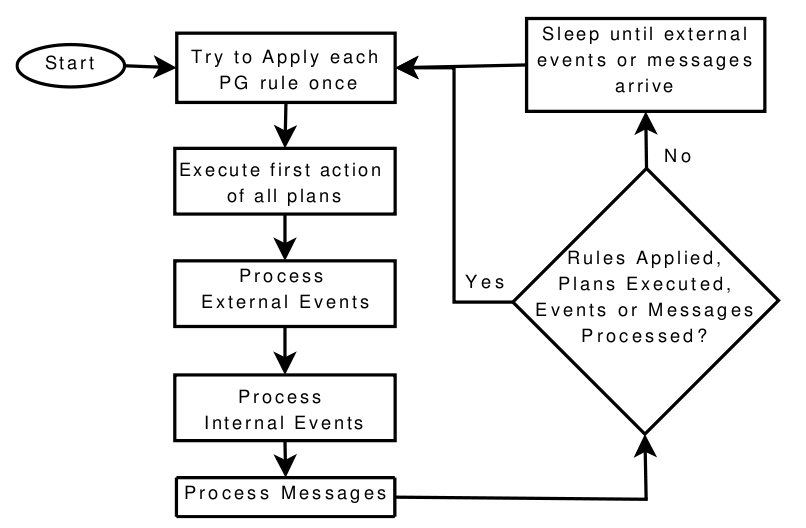
\includegraphics[keepaspectratio,scale=0.3]{fig/rcycle.png}
\end{center}

The deliberation cycle has the following two properties: first, if the execution of a plan fails, then the plan will either be repaired in the same deliberation cycle or get re-executed in the ext deliberation cycle. Second, if the first action fails and there is no plan repair rule for it, then the failed plan may be successfully executed in the next deliberation cycle.

\section{2APL Platform and Tools} %%%%%%% BORJA+MARCOS HERE

Borja+Marcos here

\section{Conclusion} %%%%%%% BORJA HERE

Borja here: conclusion + connecting with other alternatives (jadex etc)

\section{Bibliography}
\nocite{*}
\bibliographystyle{plain}
\bibliography{2apl-doc}

\end{document}
